%!TEX TS-program = xelatex
\documentclass[]{cv}
\usepackage{afterpage}
\hypersetup{hidelinks}
\usepackage{hyperref}
\usepackage{color}
\usepackage{xcolor}
\usepackage{smartdiagram}
\usepackage{fontspec}

% compile the tex file with LuaLaTeX References:
%   http://texdoc.net/texmf-dist/doc/latex/fontawesome/fontawesome.pdf
%   https://www.ctan.org/tex-archive/fonts/fontawesome?lang=en
% \usepackage{fontawesome}
\usepackage[none]{hyphenat}
\usepackage{metalogo}
\usepackage{dtklogos}
\usepackage[utf8]{inputenc}
\usepackage{tikz}
\usetikzlibrary{mindmap,shadows}

\hypersetup{
    pdftitle={},
    pdfauthor={},
    pdfsubject={},
    pdfkeywords={},
    colorlinks=false,           % no link border color
    allbordercolors=white       % white border color for all
}
\smartdiagramset{
    bubble center node font = \scriptsize,
    bubble node font = \tiny,
    % specifies the minimum size of the bubble center node
    bubble center node size = 0.4cm,
    %  specifies the minimum size of the bubbles
    bubble node size = 0.4cm,
    % specifies which is the distance among the bubble center node and the other bubbles
    distance center/other bubbles = 0.3cm,
    % sets the distance from the text to the border of the bubble center node
    distance text center bubble = 0.3cm,
    % set center bubble color
    bubble center node color = materialblue,
    % define the list of colors usable in the diagram
    set color list = {materialgreen, materialred, materialcyan, green, materialorange, materialamber, materialteal, materialindigo, materiallime, materialpurple},
    % sets the opacity at which the bubbles are shown
    bubble fill opacity = 0.4,
    % sets the opacity at which the bubble text is shown
    bubble text opacity = 0.8,
}

\addbibresource{bibliography.bib}
\RequirePackage{xcolor}
\definecolor{pblue}{HTML}{0395DE}

\begin{document}
\header{Max Liao}{}
{Software Engineer}
\par
% Fake text to add separator      
\fcolorbox{white}{gray}{\parbox{\dimexpr\textwidth-2\fboxsep-2\fboxrule}{%
	.....
}}

% In the aside, each new line forces a line break
\begin{aside} \footnotesize%
	~
	~
	~
	~
	~
	~
	~
	~
	\section{Contact \vspace{0.1cm}}
	{\small 404 314 7825 \vspace{0.05cm}}
	{\small Atlanta, GA 30345 \vspace{0.1cm}}
    {\small \href{mailto:max.liao@gmail.com}{max.liao@gmail.com} \vspace{0.05cm}}
    {\small \href{http://github.com/max-liao}{github.com/max-liao} \vspace{0.05cm}}
    {\small \href{http://www.linkedin.com/in/liao-max}{\textcolor{blue}{LinkedIn}}}%

	\section{\small Work Eligibility \vspace{0.1cm}}
	U.S. Citizen
	% use  \hspace{} or \vspace{} to change bubble size, if needed
	% \smartdiagram[bubble diagram]{
	\section{\small Computer Languages \vspace{0.05cm}}
		\textbf{Python}
		\textbf{JS, Typescript}
		\textbf{C, C\#, C++}
		\textbf{Matlab, R}
	\section{\small Web Development \vspace{0.05cm}}
		\textbf{Angular, React, Vue}
        \textbf{Node.js, Flask}
		\textbf{Electron}
		\textbf{RESTful APIs}
        \textbf{HTML5, CSS3}
		\textbf{Bootstrap, SASS}
		\textbf{Cypress, Selenium, Mocha}
	\section{\small Databases \& Backend \vspace{0.05cm}}
		\textbf{SQL}
        \textbf{MongoDB}
		\textbf{Firebase}
        \textbf{ORM (SQLAlchemy)}
    \section{\small AI \& Machine Learning \vspace{0.05cm}}
    	\textbf{Hugging Face} 
        \textbf{Vector Embeddings}
    	\textbf{Computer Vision (CV2)}
    	\textbf{TensorFlow, PyTorch}
        \textbf{NumPy, Pandas}
    	\textbf{Scikit-learn}
    	\textbf{AI Product Search}
	\section{\small DevOps}
		\textbf{Git}
        \textbf{JIRA}
		\textbf{Docker}
        \textbf{Google Cloud (GCP)}
	\section{\small Technical Skills \vspace{0.05cm}}
    	\textbf{UX/UI Design}
    	\textbf{CI/CD Testing}
    	\textbf{Technical Writing}
    	\textbf{Embedded Systems}
    	\textbf{CAD, PCB Design}
    	\textbf{3D Printing}
    	\textbf{Micro controllers}
    	\textbf{PID Controllers}
	\section{\small Languages \vspace{0.05cm}}
    	\textbf{English}
\includegraphics[scale=0.40]{img/5stars.png}
    	\textbf{Mandarin}
\includegraphics[scale=0.40]{img/4stars.png}
    	\textbf{French}
\includegraphics[scale=0.40]{img/3stars.png}
    	\textbf{Spanish}
\includegraphics[scale=0.40]{img/2stars.png}
	~
% 	\section{OS Preference \vspace{0.1cm}}
% % 	\vspace{0.1cm}
% 	\textbf{Linux}
\includegraphics[scale=0.40]{img/5stars.png}
% 	\textbf{Windows}
\includegraphics[scale=0.40]{img/4stars.png}
% 	\textbf{iOS}
\includegraphics[scale=0.40]{img/4stars.png}
	~
\end{aside}

\begin{body}
	\section{\vspace{0.05cm} Highlights}
    	\begin{itemize}
            \item {Senior software engineer with 7 years of experience in designing and developing robust and user-friendly applications}
            \item {Built applications with automated data collection pipelines and integrated AI models, including computer vision for image-based classification and similarity matching}
            \item {Experience with Agile Software Development and CI/CD methodologies}
    	\end{itemize}
        \vspace{0.075cm}
	\section{Experience}
    	\begin{entrylist}
    		\entry
    		{03/19 - now}
    		{Software Engineer}
    		{TKE}
    		{Responsible for touchscreen elevator dispatch system software used on elevator kiosks, car operating panels, and smart mirrors
    			\begin{itemize}
                    \item {Fully upgraded application from AngularJS to modern Angular}
                    \item {CI/CD - added Cypress testing and integrated reporting with JIRA }
                    \item {Implemented cybersecurity upgrades including CSP, strict password enforcement, and session security hardening}
    				\item {Created ElectronJS app using Vue to simulate destination dispatch of elevators using RS-485 and UDP}
    			\end{itemize}
            }
    		\entry 
    		{11/18 - 6/19}
    		{Teacher's Assistant}
    		{Georgia Institute of Technology}
    		{Full Stack Flex Web Development - teacher's assistant with Trilogy Education\\
    		Taught night classes for Georgia Tech Professional Education\\
    	    Material included NodeJS, ExpressJS, SQL/MongoDB, React}
    		\entry
    		{4/18 - 12/18}
    		{Software Engineer}
    		{NCR Corporation}
    		{Software and firmware support for the ATM hardware division at NCR \\
    		Created and supported analysis tool for the Scalable Deposit Module 2}
    		\entry
    		{8/15 - 12/17}
    		{Research Assistant}
    		{Skidaway Institute of Oceanography}
    		{Researched UV-wet chemical oxidation dissolved organic carbon (DOC) analyzer for aqueous samples to obtain higher precision, faster speeds, and more adaptable usage than commercial instruments
    		}		  
          \entry
          {4/15 - 9/15}
          {Electrical Engineer}
          {PhytoSynthetix}
          {Made improvements to a fluorometer for grow chamber monitoring at the University of Georgia horticultural greenhouse}
          \entry
          {1/13 - 1/15}
          {Software Test Engineer}
          {Cisco Systems}
          {Install and maintain a continuous integration test framework for set top boxes
          	\begin{itemize}
          		\item {Developed test software and procedures in Python and C}
          		\item {Generated specification and prototype test equipment per product test and repair requirements}
          	\end{itemize}
          }
        \end{entrylist}
        \vspace{0.05cm}
	\section{Education}
        \vspace{0.05cm}
		\begin{entrylist}
			\entry
    			{2015 - 2017}
    			{Master of Science in Biological Engineering}
    			{University of Georgia}
    			{Research Assistant at Skidaway Institute of Oceanography \newline Certificate in Coastal and Oceanographic Engineering
    				\begin{description}
    					\item {Advisers: Dr. Aron Stubbins and Dr. Mark Haidekker}
    				\end{description}}
			\entry
    			{2008 - 2012}
    			{Bachelor of Science in Electrical Engineering}
    			{Georgia Institute of Technology}
    			{Undergraduate Research Opportunities Program
    				\begin{description}
    					\item {Adviser: Dr. Manos Tentzeris}
    				\end{description}
                }
    		\entry
        		{2018}
        		{Full Stack Flex Web Development}
        		{Georgia Institute of Technology}
        		{Georgia Tech Professional Education coding bootcamp}
		\end{entrylist}
\end{body}
\end{document}
% \newpage
% 	\section{Certifications\\}
%     	\begin{entrylist}
%     		\entry
%     		{08/2018}
%     		{Full Stack Flex Web Development}
%     		{Georgia Institute of Technology}
%     		{Professional education certificate for a full stack web development coding bootcamp}
%     		\entry
%     		{12/2017}
%     		{Coastal and Oceanographic Engineering}
%     		{University of Georgia}
%     		{Graduate certificate for multi-disciplinary program in engineering and marine sciences emphasizing marine instrumentation and numerical modeling of near-shore and coastal processes\\ Includes course work in engineering and marine sciences as well as a research and design component at the graduate level}
%     	\end{entrylist}
% % 	\section{Other Info}
% %     	~
% %     	Can read/write French and Spanish\\
% %     	\emph{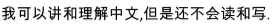
\includegraphics[scale=1]{img/Chinese.PNG}}\\
% % 	\section{Publications}
% %     	Max Liao\\ \textbf{A Precision UV-Wet Chemical Oxidation Dissolved Organic Carbon Analyzer}\\
% %     	MS Thesis. University of Georgia, 2017
% %     	\\\\
% %     	Wenting Gu, Peng Cheng, Arindam Ghosh, Max Liao, Boxiong Liao, Ali Beskok, Zhili Hao\\
% %     	\textbf{Detection of distributed static and dynamic loads with electrolyte enabled distributed transducers in a polymer based microfluidic device}\\
% %     	\emph{ Journal of Micromechanics and Microengineering, Vol. 23, March 2013, 035015 (15pp), doi:10.1088/09601317/23/3/035015 (featured in IOPselect) }
% %     	\\\\
% %     	Wenting Gu, Peng Cheng, Arindam Ghosh, Max Liao, Boxiong Liao, Ali Beskok, Zhili Hao\\
% %     	\textbf{A polymer based microfluidic resistive sensor for detecting distributed loads}\\
% %     	\emph{ ASME International Mechanical Engineering Congress and Exposition (IMECE2012), \\ Nov. 9-15, 2012, Houston, Texas, IMECE201287672 (Best Paper Award in the MEMS Division) }
% %     	\\
% %     	\begin{flushleft}
% %     	\end{flushleft}
%     	\begin{flushright}
%     		\emph{Max Liao }
%     		\emph{Software Engineer}
%     	\end{flushright}
% \end{body}
% \begin{aside}
% ~
% 	~
% 	~
% 	\section{Languages}
% 	~
% 	\textbf{English}
\includegraphics[scale=0.40]{img/5stars.png}
% 	\textbf{Mandarin}
\includegraphics[scale=0.40]{img/4stars.png}
% 	\textbf{French}
\includegraphics[scale=0.40]{img/3stars.png}
% 	\textbf{Spanish}
\includegraphics[scale=0.40]{img/2stars.png}
% 	~
% \end{aside}
% \end{document}